%%%%%%%%%%%%%%%%%%%%%%%%%%%%%%%%%%%%%%%%%%%%%%%%%%%%%%%%%%%%
%%% LIVECOMS ARTICLE TEMPLATE FOR BEST PRACTICES GUIDE
%%% ADAPTED FROM ELIFE ARTICLE TEMPLATE (8/10/2017)
%%%%%%%%%%%%%%%%%%%%%%%%%%%%%%%%%%%%%%%%%%%%%%%%%%%%%%%%%%%%
%%% PREAMBLE
\documentclass[9pt,bestpractices]{livecoms}
% Use the 'onehalfspacing' option for 1.5 line spacing
% Use the 'doublespacing' option for 2.0 line spacing
% Use the 'lineno' option for adding line numbers.
% Use the "ASAPversion' option following article acceptance to add the DOI and relevant dates to the document footer.
% Use the 'pubversion' option for adding the citation and publication information to the document footer, when the LiveCoMS issue is finalized.
% The 'bestpractices' option for indicates that this is a best practices guide.
% Omit the bestpractices option to remove the marking as a LiveCoMS paper.
% Please note that these options may affect formatting.

\usepackage{lipsum} % Required to insert dummy text
\usepackage[version=4]{mhchem}
\usepackage{siunitx}
\DeclareSIUnit\Molar{M}
\usepackage[italic]{mathastext}
\graphicspath{{figures/}}

%% GOOGLE DOCS WHERE ORIGINAL OUTLINE WAS: https://docs.google.com/document/d/1lCGcol6jYLQmcfqrUv9h_FsWygTZzqYxqgjOLCyMoL4/edit

%%%%%%%%%%%%%%%%%%%%%%%%%%%%%%%%%%%%%%%%%%%%%%%%%%%%%%%%%%%%
%%% IMPORTANT USER CONFIGURATION
%%%%%%%%%%%%%%%%%%%%%%%%%%%%%%%%%%%%%%%%%%%%%%%%%%%%%%%%%%%%

\newcommand{\versionnumber}{0.1}  % you should update the minor version number in preprints and major version number of submissions.
\newcommand{\githubrepository}{\url{https://github.com/openforcefield/FE-Benchmarks-Best-Practices}}  %this should be the main github repository for this article

%%%%%%%%%%%%%%%%%%%%%%%%%%%%%%%%%%%%%%%%%%%%%%%%%%%%%%%%%%%%
%%% ARTICLE SETUP
%%%%%%%%%%%%%%%%%%%%%%%%%%%%%%%%%%%%%%%%%%%%%%%%%%%%%%%%%%%%
\title{Best practices for constructing, preparing, and evaluating protein-ligand binding affinity benchmarks [Article v\versionnumber]}
\author[1*]{David Hahn}
\author[2]{Hannah E. Bruce Macdonald}
\author[3]{Laura Perez Benito}
\author[2]{John D. Chodera}
\author[4]{Antonia S. J. S. Mey}
\author[5]{David L. Mobley}
\author[6]{Gary Tresadern}
\author[1,2\authfn{1}\authfn{3}]{Firstname Middlename Familyname}
\author[2\authfn{1}\authfn{4}]{Firstname Initials Surname}
\affil[1]{Institution 2}
\affil[2]{Computational and Systems Biology Program, Sloan Kettering Institute, Memorial Sloan Kettering Cancer Center, New York, NY 10065}
\affil[3]{Institution 2}
\affil[4]{Institution 2}
\affil[5]{Departments of Pharmaceutical Sciences and Chemistry, University of California, Irvine, CA USA}
\affil[6]{EaStCHEM School of Chemistry, David Brewster Road, Joseph Black Building, The King's Buildings, Edinburgh, EH9 3FJ, UK}
\affil[2]{Institution 2}

\corr{email1@example.com}{FMS}  % Correspondence emails.  FMS and FS are the appropriate authors initials.
\corr{email2@example.com}{FS}

\orcid{Author 1 name}{AAAA-BBBB-CCCC-DDDD}
\orcid{Hannah E. Bruce Macdonald}{0000-0002-5562-6866}
\orcid{Author 3 name}{AAAA-BBBB-CCCC-DDDD}

\contrib[\authfn{1}]{These authors contributed equally to this work}
\contrib[\authfn{2}]{These authors also contributed equally to this work}

\presentadd[\authfn{3}]{Department, Institute, Country}
\presentadd[\authfn{4}]{Department, Institute, Country}

\blurb{This LiveCoMS document is maintained online on GitHub at \githubrepository; to provide feedback, suggestions, or help improve it, please visit the GitHub repository and participate via the issue tracker.}

%%%%%%%%%%%%%%%%%%%%%%%%%%%%%%%%%%%%%%%%%%%%%%%%%%%%%%%%%%%%
%%% PUBLICATION INFORMATION
%%% Fill out these parameters when available
%%% These are used when the "pubversion" option is invoked
%%%%%%%%%%%%%%%%%%%%%%%%%%%%%%%%%%%%%%%%%%%%%%%%%%%%%%%%%%%%
\pubDOI{10.XXXX/YYYYYYY}
\pubvolume{<volume>}
\pubissue{<issue>}
\pubyear{<year>}
\articlenum{<number>}
\datereceived{Day Month Year}
\dateaccepted{Day Month Year}

%%%%%%%%%%%%%%%%%%%%%%%%%%%%%%%%%%%%%%%%%%%%%%%%%%%%%%%%%%%%
%%% ARTICLE START
%%%%%%%%%%%%%%%%%%%%%%%%%%%%%%%%%%%%%%%%%%%%%%%%%%%%%%%%%%%%

%% GOOGLE DOCS WHERE ORIGINAL OUTLINE WAS: https://docs.google.com/document/d/1lCGcol6jYLQmcfqrUv9h_FsWygTZzqYxqgjOLCyMoL4/edit

\begin{document}

\begin{frontmatter}
\maketitle

\begin{abstract}
Free energy simulations are rapidly becoming a key component to the drug design process and significant efforts have been made to streamline these methods for ease of application. As these tools become more widespread and new innovations in methods and force fields are developed, benchmarking of the performance of free energy calculations on real-world systems becomes critical so that downstreams users can have an idea of what level of accuracy is to be expected. Such benchmarking, however, requires construction of well prepared, high quality benchmark sets in order to ensure they provide a realistic assessment of performance. However, the accuracy of results also dependsuseful results are reliant on the set up of the benchmark systems themselves, such as choices made in protein preparation. Diverse choices made in analysis can also impact apparent performance. Here, we address these critical issues by presenting guidelines for selecting good experimental datasets to serve as benchmarks for free energy calculations in order to assess real-world performance as well as possibly identify challenges that remain to be solved. We also give guidelines for preparing systems for binding free energy calculations such as for in benchmarking tests, and make recommendations as to how to analyze the performance of the resulting predictions and draw conclusions about relative performance of different techniques or methods. This work provides a summary of the practices we plan to use in our own benchmarking work on free energy calculations, as well.
\end{abstract}

\end{frontmatter}




\section{Introduction}

Here you would explain what problem you are tackling and briefly motivate your work.

In this particular template, we have removed most of the usage examples which occur in \texttt{sample-document.tex} to provide a minimal template you can modify; however, we retain a couple of examples illustrating more unusual features of our templates/article class, such as the checklists, and information on algorithms and pseudocode.

Keep in mind, as you prepare your manuscript, that you should plan for a representative image  which will be used to highlight your article on the journal website and publications. Usually, this would be one of your figures, but it must also be uploaded separately upon article submission. We give specific guidelines for this image on the journal website in the section on article submission (see \url{https://livecomsjournal.github.io/authors/policies/index.html#article-submission}).

Additionally, for well-formatted manuscripts, we recommend that you let LaTeX handle figure/table placement for you as much as possible, so please avoid specifying strenuous float instructions like `[h!]` and `[H]` as much as possible.

\section{Prerequisites}

Here you would identify prerequisites/background knowledge that are assumed by your work and your checklist which you view as critical, ideally giving links to good sources on these topics.
Checklists are normally focused on errors made by users with training and experience in molecular simulations, so you can assume a basic familiarity with the fundamentals of molecular simulations.

\section{Checklist}
Here we use a full-page checklist with multiple sections, so it will appear on a separate page of the sample PDF.
Other checklist formats are possible, as shown in the sample \texttt{sample-document.tex} in \url{github.com/livecomsjournal/article_templates/templates}.

Your checklist should include a succinct list of steps that people should follow when carrying out the task in question.
This is provided to ensure certain basic standards are followed and common but critical major errors are avoided.
Note that a checklist is not intended to cover \emph{all} important steps, but rather focus on the most common reasons for failure or incorrect results, or issues which are particularly crucial.


% This provides a checklist which
% - spans a full page
% - consists of multiple sub-checklists
% - exists on a separate page
% This style of checklist will be especially helpful if you want to encourage readers to print and use your checklist in practice, as they
% can easily print it without also printing other material from your manuscript. However, other styles of checklist are also possible (below).

\begin{Checklists*}
\begin{checklist}{Second list}
\textbf{This is some further description.}
\begin{itemize}
\item First thing
\item Also remember
\item And finally
\end{itemize}
\end{checklist}

\begin{checklist}{Third list}
\textbf{This is some further description.}
\begin{itemize}
\item First thing
\item Also remember
\item And finally
\end{itemize}
\end{checklist}

\begin{checklist}{Plotting results}
\textbf{Presenting results in an appropriate format: Section~\ref{sec:plotting_results}}
\begin{itemize}
\item Clearly label the data with titles, legends, and captions.
\item Plot results with the dependent variable (calculated) on y-axis, and the independent variable (experimental) on the x-axis. 
\item Ensure that the data are reported in the same units on both axes, and labelled. Where the units are consistent, the scale of the axis in real space should be consistent, such that a 1 cm change on the x-axis corresponds to the same change in affinity to 1 cm on the y-axis.
\item Plot only one target per plot, unless specifically looking at selectivity.
\end{itemize}
\end{checklist}

\begin{checklist}{Statistical analysis}
\textbf{Quantifying the success of a method: Section~\ref{sec:statistical_analysis}}
\begin{itemize}
\item 
\item Identify which metrics are appropriate for your method. Statistics that measure accuracy, such as RMSE and MUE are commonplace, and additionally correlation statistics are appropriate for absolute free energies, but not relative free energies.
\item Bootstrap statistics to provide confidence intervals. 
\end{itemize}
\end{checklist}


\end{Checklists*}





\section{Rationale}

Your Rationale section, or sections, can follow or precede your checklist (we expect that often, following the checklist will be preferable) and provide the necessary rationale for the checklist, and act as more complete \emph{best practices} description.
This should include 1) significant detail as to the possible alternative ways to accomplish a given task, 2) description of advantages and disadvantages of the various approaches, and 3) significant literature documentation about reasons for choices.

\subsection{Algorithms and Pseudocode}
\label{sec:reference_this}

The \texttt{algpseudocode} and \texttt{algorithms} packages is loaded by the document class. \ALG{euclid} was taken directly from the package documentation. (Please do not load \texttt{algorithm2e}; it's not compatible with \texttt{algpseudocde} nor \texttt{algorithms}!)

\begin{algorithm}
\caption{Euclid's algorithm}\label{alg:euclid}
\begin{algorithmic}%[1]  %% uncomment to enable line numbers
\Procedure{Euclid}{$a,b$}\Comment{The g.c.d. of a and b}
   \State $r\gets a\bmod b$
   \While{$r\not=0$}\Comment{We have the answer if r is 0}
      \State $a\gets b$
      \State $b\gets r$
      \State $r\gets a\bmod b$
   \EndWhile\label{euclidendwhile}
   \State \textbf{return} $b$\Comment{The gcd is b}
\EndProcedure
\end{algorithmic}
\end{algorithm}


\subsection{dataset selection}


\subsubsection{structural data}
\label{sec:struct_data}
\begin{Checklists*}[p!]

\begin{checklist}{Structural Data}
\textbf{This list of items will go to Sect. \ref{sec:struct_data}}
\begin{itemize}
\item a successful free energy calculation requires are well prepared model of the system, with structures close to its energetic minimum. the basis for this is an experimental structure, either from X-ray crystallography, cryo EM, NMR or homology models. https://doi.org/10.1021/acs.jcim.7b00564, https://doi.org/10.1021/acs.jcim.0c00116; https://doi.org/10.26434/chemrxiv.11364884.v2; 
\item quality of x-ray structure  (Iridium: https://doi.org/10.1016/j.drudis.2012.06.011)
    \begin{itemize}
    \item Global criteria
        \begin{itemize}
        \item x-ray resolution only gives a theoretical limit, therefore not a good metric for quality. it should be < 2.0 (Schindler et al.) or < 3.5 (Warren et al) $\AA$
        \item Use coordinate error to select the best structure (< 0.7)
        \item Experimental data is available, i.e. electron density
        \item The reported Rfree < 0.45 when resolution $\ge 3.5 \AA$
        \item The reported difference between R and Rfree $\ge 0.05$
        \end{itemize}
    \item Local criteria
        \begin{itemize}
        \item Identify ligand atoms where there are crystal packing atoms within 6 Å
        \item The ligand must have at least partial density (check visually or RSCC > 0.80)
        \item All ligand and active site atoms with occupancy <1.0 are identified
        \item Active site atoms with partial density are identified
        \item Also are crystallographic waters resolved
        \item Alternate conformations for ligand and active site atoms are identified
        \item Identify covalent ligands
        \item Are there crystal contacts? 
        \item  Local metrics such as EDIA or Zobs or Spruce(?) can indicate if the electron density is sufficient to support the crystallographic placement of a given atom.
        \end{itemize}
    \end{itemize}
\item aspects to be considered beyond the quality of the structure (see also structure preparation, Sect. \ref{sec:prep}
    \begin{itemize}
    \item Structure (also the binding mode!) could be deformed due to crystal contacts, additives, experimental temperature,... Can you assume the structure in the crystalline form is representative of the biologically active conformation? 
    \item Content of the structure: is the small molecule (or a closely related one) bound? 
    \item Are there cofactors or cobinders which should be included to model the natural environment of the protein?
    \item Can we model the measurement conditions, temperature, ion concentration, other additives?
    \item Can we model the natural environment (ion concentration, cofactors, membranes, ...)?
    \end{itemize}
\item If these requirements are not met, it does not necessarily mean that the data is not usable and  the results will be bad. A structure not meeting the requirements just needs more manual work by --- ideally an experienced --- user. Unresolved areas can be modelled with nowadays tools and knowledge about atom interactions.
\item Collective intelligence could be a way to mitigate the influence of individuals to the prepared input structures of a benchmark set. On a platform, other scientists could suggest changes to structures and updated versions could be deposited, increasing the quality of the benchmark set. Endorsement and rating of deposited structures could increase the trust into specific structures and the database in general. 
\end{itemize}
\end{checklist}

\end{Checklists*}

\subsubsection{binding data}

\subsection{setting up simulations}

\subsubsection{Structure preparation}
\label{sec:prep}

\subsection{Measuring the success of free energy calculations requires careful analysis}
Reliable reporting and analysis of the success of calculations is vital for the validation and benchmarking of free energy methods as well as the dissemination of published results. This reporting and analysis falls into two major categories -- plotting or visualization of results, and statistical analysis of the results. Here we make recommendations for both categories.

\subsubsection{Plots of free energy results should adhere to certain common standards}
\label{sec:plotting_results}
Figures plotting experimental vs. calculated results are a very useful way to gauge the success of a method or a set of calculations. We recommend several key steps to ensure these plots are valuable, communicate accurate information, and are informative and readable. Experimental values (on the x-axis) should be converted into the same units as the free energy results (on the y-axis), and axes should use the same scale. One common issue with plotting free energy results is that different scales are used on the different axes, which can change the appearance of the results.

\begin{figure}
    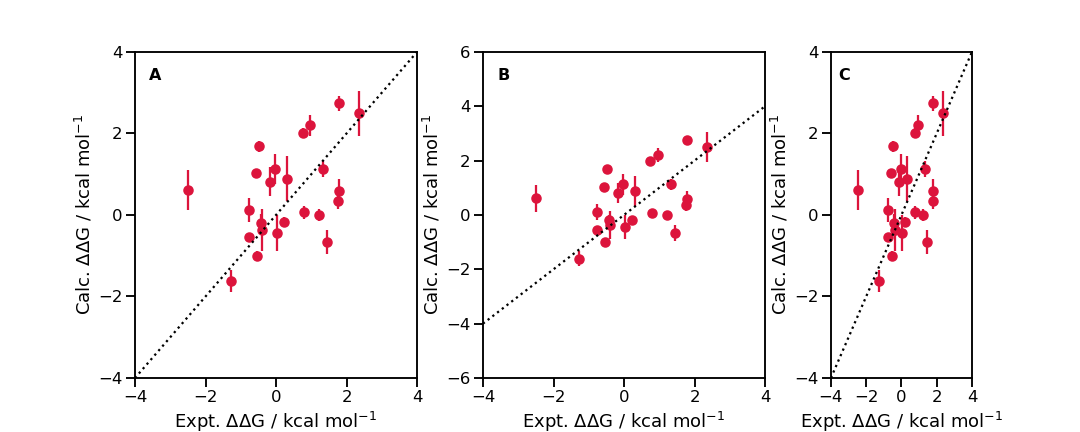
\includegraphics[width=0.95\linewidth]{figures/plotting-basics.png}
    \caption{\textbf{Changes to the plotting style can change the appearance of the data.} The above three figures illustrates the same toy data. A) shows the data correctly, with the same units (which are labelled) and scales on both axes. B) shows the same data, however the limits on the y-axis have been changed such that the scales is not consistent. C) is also not consistent, but this is due to the scale of the plot, rather than the limits.}
    \label{fig:plotting-basics}
\end{figure}

Error bars can be very helpful in understanding the uncertainty in the data -- both for calculated values and for experimental values, and thus both experimental and computational error bars should always be included in visualizations of the data. Different sources of error might be used to quantify this, whether an uncertainty directly from a free energy estimator, variance between repeats or a hysteresis-type analysis. How the error bars have been calculated should be reported in the figure caption.\\
* more details on ways to compute error bars?\\
* more details on experimental error bars?\\
Additionally, experimental values which were not actually measured (e.g. values resulting from a measured $K_D$ value which only has experimental bounds, such as $> 5 \mu M$) should not be plotted or should be clearly indicated by different styles and symbols.

Finally, plots of results across various targets should typically show one figure per target. Differences in the success of free energy methods can vary widely between targets, and combining the data across targets onto a single plot can obscure actual performance on any given target. Additionally, when considering absolute free energies, the affinity ranges between targets may vary, which may result in analysis picking up the correlation between targets and their affinities, rather than the free energy methods ability to differentiate affinities for a particular target. One exception to this however may be if free energy calculations were being performed for selectivity analysis of similar proteins, whereby the targets are not independent parameters.

\subsubsection{Consistent reporting of statistics is vital for measuring success}
\label{sec:statistical_analysis}
Free energy calculations fall into two categories: absolute and relative. Depending on which type of result are being analyzed --- absolute or relative --- different statistics will be appropriate. Accuracy statistics, such as root mean squared error (RMSE) and mean unsigned errors (MUE) provide information as to how well the computational method recapitulates the experimental results, and allow for a 'best guess' as to how far the computation prediction of new ligands' affinities may be from experiment. Correlation statistics, such as $R^{2}$, Kendall tau ($\tau$) and Spearman's rank ($\rho$) indicate how well a method does at ordering the results, at identifying the best and worst ligand in a set, which in live drug design projects where these models may be used to make purchasing decisions, may be a more useful metric than accuracy.\\

One mistake that is commonly made, is the use of correlation-type statistics for the bench marking of relative free energy calculations. As relative calculations are pairwise comparisons between ligands, the direction, or sign of the calculation is arbitrary. If a ligand $A$ is 2 kcal mol $^{-1}$ higher affinity than ligand $B$, this could equally be plotted and reported as ligand $B$ being -2 $kcal mol ^{-1}$ lower affinity than ligand $A$. The consequence of the possible inversion of data points can shift the correlation statistics, despite the underlying data being reliable. The same set of data points can give a range of statistical results depending on arbitrary sign-flips in the data set. While this effect is reduced with increasing data set size, this can still be problematic. If a clear protocol is used, such as mapping all of the results to either be all positive or all negative, or plotting both $A$ -> $B$ and $B$ -> $A$ then the statistics quoted will be reproducible, however is possibly best to avoid correlation statistics for relative free energy results.



* more details on other analysis methods GRAM RRMSE etc. etc. 


\subsubsection{Bootstrapping is a reliable method for determining confidence intervals for statistics}

While statistics are a useful measure of the performance of a method, it is also important to understand how accurate those measures are themselves. Is a MUE of 1.2 kcal mol$^{-1}$ much better than 1.3 kcal mol$^{-1}$? Would the performance be likely to change on the addition of new ligands in the series? Is the R$^2$ being heavily leveraged by a few outliers? Performing bootstrap analysis allows for confidence intervals to be placed on the statistics, and for these questions to be answered with some confidence. A MUE of 1.2 (0.6) kcal mol$^{-1}$ is not statistically different than a MUE of 1.3 (0.5) kcal mol$^{-1}$. Bootstrap analysis provides a measure of accuracy to the statistics through random sampling with replacement. Bootstrapping should be performed on the data used to compute the statistic reported --- for relative free energies this illustrate how sensitive the statistics are to the edges chosen, and for absolute free energies: the sensitivity to the ligands in the set. If a statistical error is available for each data-point, such as the error afforded from the free energy estimator, then this can be incorporated into the bootstrap estimate, by bootstrapping over a sample taken from each datapoint with it's associated error.\\
How many bootstraps do you need to do to converge?\\
It is best practise to report the bootstrapped statistical errors alongside data as 95\% confidence intervals to appropriately evaluate the performance of a particular method, and identify if improvements or changes to a model are statistically significant.


\section{Author Contributions}
%%%%%%%%%%%%%%%%
% This section mustt describe the actual contributions of
% author. Since this is an electronic-only journal, there is
% no length limit when you describe the authors' contributions,
% so we recommend describing what they actually did rather than
% simply categorizing them in a small number of
% predefined roles as might be done in other journals.
%
% See the policies ``Policies on Authorship'' section of https://livecoms.github.io
% for more information on deciding on authorship and author order.
%%%%%%%%%%%%%%%%

(Explain the contributions of the different authors here)

% We suggest you preserve this comment:
For a more detailed description of author contributions,
see the GitHub issue tracking and changelog at \githubrepository.

\section{Other Contributions}
%%%%%%%%%%%%%%%
% You should include all people who have filed issues that were
% accepted into the paper, or that upon discussion altered what was in the paper.
% Multiple significant contributions might mean that the contributor
% should be moved to authorship at the discretion of the a
%
% See the policies ``Policies on Authorship'' section of https://livecoms.github.io for
% more information on deciding on authorship and author order.
%%%%%%%%%%%%%%%

(Explain the contributions of any non-author contributors here)
% We suggest you preserve this comment:
For a more detailed description of contributions from the community and others, see the GitHub issue tracking and changelog at \githubrepository.

\section{Potentially Conflicting Interests}
%%%%%%%
%Declare any potentially competing interests, financial or otherwise
%%%%%%%

Declare any potentially conflicting interests here, whether or not they pose an actual conflict in your view.

\section{Funding Information}
%%%%%%%
% Authors should acknowledge funding sources here. Reference specific grants.
%%%%%%%
FMS acknowledges the support of NSF grant CHE-1111111.

\section*{Author Information}
\makeorcid

\bibliography{livecoms-sample}

%%%%%%%%%%%%%%%%%%%%%%%%%%%%%%%%%%%%%%%%%%%%%%%%%%%%%%%%%%%%
%%% APPENDICES
%%%%%%%%%%%%%%%%%%%%%%%%%%%%%%%%%%%%%%%%%%%%%%%%%%%%%%%%%%%%

%\appendix


\end{document}
